\documentclass[english,compress]{beamer}
\usepackage{kloeckislides}
\nonstopmode

\usepackage[normalem]{ulem}
\usepackage{pifont}
\usepackage{ifthen}

\setbeamercolor{section in head/foot}{use=structure,bg=structure.fg!25!bg}
\defbeamertemplate*{footline}{split theme}
{%
  \leavevmode%
  \begin{beamercolorbox}[wd=.5\paperwidth,ht=2.5ex,dp=1.125ex]{section in head/foot}%
    \insertsectionnavigationhorizontal{\paperwidth}{\hskip0pt plus1filll}{}%
  \end{beamercolorbox}%
  %\begin{beamercolorbox}[wd=.5\paperwidth,ht=2.5ex,dp=1.125ex]{subsection in head/foot}%
    %\insertsubsectionnavigationhorizontal{.5\paperwidth}{}{\hskip0pt plus1filll}%
  %\end{beamercolorbox}%
}


%\useoutertheme[subsection=false]{miniframes}

\setbeamertemplate{frametitle}[default][center]

\AtBeginDocument{%
  {
    \usebeamercolor{section in head/foot}
  }
  
  \pgfdeclareverticalshading{beamer@headfade}{\paperwidth}
  {%
    color(0cm)=(bg);
    color(1.25cm)=(section in head/foot.bg)%
  }

  \setbeamercolor{section in head/foot}{bg=}
}

\addtoheadtemplate{\pgfuseshading{beamer@headfade}\vskip-1.25cm}{}

\beamertemplatedotitem

\setbeamercolor{section in head/foot}{parent=palette quaternary}
\setbeamercolor{subsection in head/foot}{parent=palette primary}

\setbeamercolor{author in head/foot}{parent=section in head/foot}
\setbeamercolor{title in head/foot}{parent=subsection in head/foot}



\AtBeginSection[] {
  \begin{frame}<beamer>
  \frametitle{Outline}
  \tableofcontents[sectionstyle=show/shaded,subsectionstyle=show/show/hide]
\end{frame}
}
\AtBeginSubsection[] {
  \begin{frame}<beamer>
  \frametitle{Outline}
  \tableofcontents[sectionstyle=show/shaded,subsectionstyle=show/shaded/hide]
\end{frame}
}

\newcommand{\technicality}[2]{%
  {\strut #1\\
    \begin{beamercolorbox}[sep=1mm]{block body}
      #2
    \end{beamercolorbox}
  }%
}

\lstset{
  language=C++,
  rangebeginprefix=//\ ,
  rangeendprefix=//\ ,
}

\def\weblink#1#2{\href{#1}{\color{blue}\underline{#2}}}

\definecolor{fetch}{RGB}{227,110,35}
\definecolor{alu}{RGB}{255,188,24}
\definecolor{context}{RGB}{132,146,175}

\usepackage{keystroke}

\setbeamertemplate{navigation symbols}{}


\begin{document}
% {{{ front matter

\title{High-Performance Scientific Computing\\Lecture 1: Intro}

\date{MATH-GA 2011 / CSCI-GA 2945 $\cdot$ September 5, 2012}

\frame{\titlepage}

\begin{frame}{Today}
  \tableofcontents[hideallsubsections]
\end{frame}
% }}}
% -----------------------------------------------------------------------------
\section{About this class}
% -----------------------------------------------------------------------------
% {{{
% -----------------------------------------------------------------------------
\begin{frame}{Course Goal}

  \begin{center}
    \Large
    Slow code goes in.

    \Huge
    Speedy code goes out.
  \end{center}

  \hrulefill

  \bigskip
  Learn about:
  \begin{itemize}
    \item Machines
    \item Tools / Languages
    \item Algorithms / Ways of thinking
    \item Important examples
  \end{itemize}
\end{frame}
% -----------------------------------------------------------------------------
\begin{frame}{Define slow?}
  \begin{columns}
    \column{0.6\textwidth}
    \only<1>{
      \movie[width=\textwidth,height=0.85\textwidth,poster]{}
      {../lec1-media/ka6d-contour.webm}
    }
    \only<2->{
      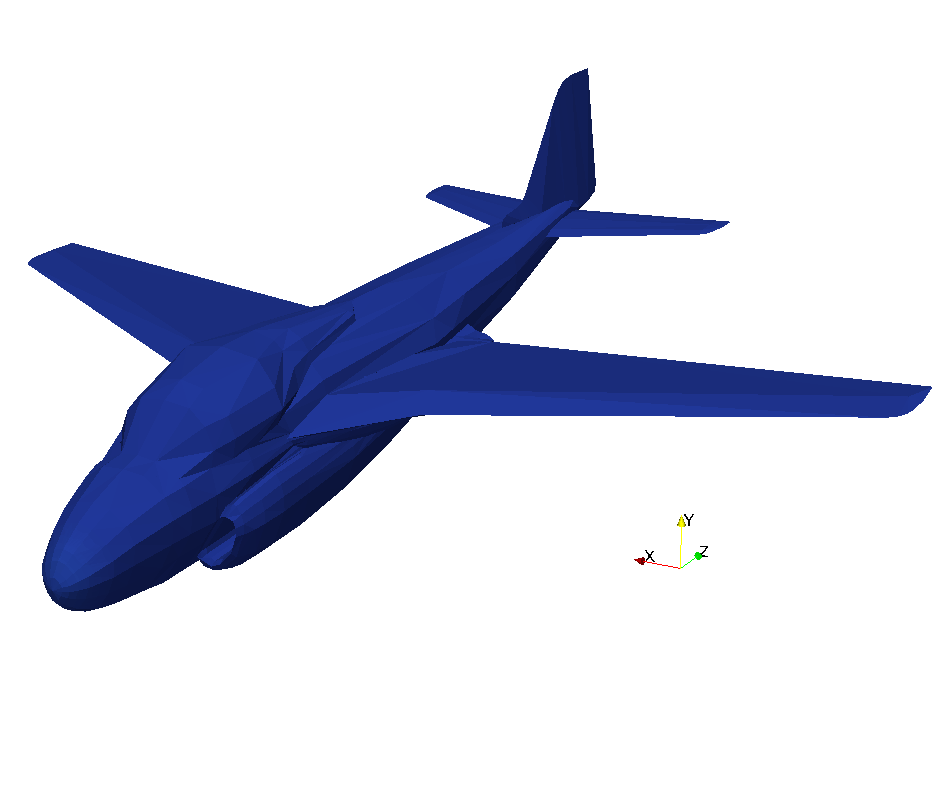
\includegraphics[width=\textwidth]{ka6d-contour.png}
    }
    \column{0.4\textwidth}
    \pause
    \begin{itemize}[<+->]
      \item Takes about 30 days on a single PC.
      \item Takes about a day on a GPU.
    \end{itemize}

    \uncover<+->{
      That's still pretty crude-looking.
    }

    \medskip
    \uncover<+->{
      Suppose I'd like to double the resolution. (i.e. cut the mesh
      width $h$ in half.)
    }
    \vspace{-2ex}
    \begin{itemize}[<+->]
      \item Had $K$ elements. Now?
      \item Anything else?
      \item $16\times$ the cost!
    \end{itemize}

  \end{columns}
  \uncover<+->{
    \begin{tikzpicture} [overlay]
      \node [above right=10mm of current page.south west,
        draw,drop shadow,fill=white,inner sep=5mm,thick,
        text width=6cm]
        {
          Well, how about 16 GPUs then?

          \bigskip
          \only<+->{
            $\rightarrow$ Realistic (high-fidelity) problems are big.
          }

          \medskip
          \only<+->{
            $\rightarrow$ You'll need a bigger hammer.
          }

          \medskip
          \only<+>{%
            \textbf{%
            You'll need to know \emph{how to use} the bigger hammer.
          }
          }
        } ;
    \end{tikzpicture}
  }
\end{frame}
% -----------------------------------------------------------------------------
\begin{frame}{Course Outline}
  \begin{tikzpicture}[overlay]
    \node [above left =1cm of current page.south east,
    rotate=10,opacity=0.3,yshift=1cm] 
    { \includegraphics[width=8cm]{dictionary.jpeg} } ;
  \end{tikzpicture}
  \begin{columns}
    \column{0.5\textwidth}
    \textbf{Part 1: Do} ($\sim 4$)

    \begin{itemize}
      \item Write, run programs (C)
      \item Use tools (make, git, gdb)
      \item OpenMP, MPI, OpenCL
      \item Correctness in each
    \end{itemize}

    \medskip
    \textbf{Part 2: Understand} ($\sim$3)

    \begin{itemize}
      \item Measure and understand performance
      \item Basic machine architecture
      \item CPU machine model
      \item GPU machine model
    \end{itemize}

    \column{0.5\textwidth}
    \textbf{Part 3: Refine} ($\sim$3)

    \begin{itemize}
      \item Advanced tools \& languages
      \item Work partitioning
      \item Common patterns
      \item Load balancing
    \end{itemize}

    \medskip
    \textbf{Part 4: Apply}

    \begin{itemize}
      \item Find a project\\
        (start looking \emph{now}!)
      \item Pitch it to us (5 min)
      \item Apply what you've learned
      \item Present your work (2)
    \end{itemize}
  \end{columns}
\end{frame}
% -----------------------------------------------------------------------------
\begin{frame}{Sign-up sheet}
  \begin{center}
    \includegraphics[height=7cm]{notebook.jpeg}
  \end{center}
\end{frame}
\addimgcredit{Notebook: sxc.hu/abeall}
% -----------------------------------------------------------------------------
\begin{frame}{Survey}
  \begin{columns}
    \column{0.5\textwidth}
    \includegraphics[width=\textwidth]{question-mark.jpeg}
    \column{0.5\textwidth}
    \begin{itemize}[<+->]
      \item Home department
      \item Degree
      \item Longest program ever written?
      \item Language?
      \item Parallel?
      \item Already have a project?
    \end{itemize}
  \end{columns}
\end{frame}
\addimgcredit{Question mark: sxc.hu/svilen001}
% -----------------------------------------------------------------------------
\begin{frame}{Class web page}
  \begin{columns}
    \column{0.6\textwidth}
      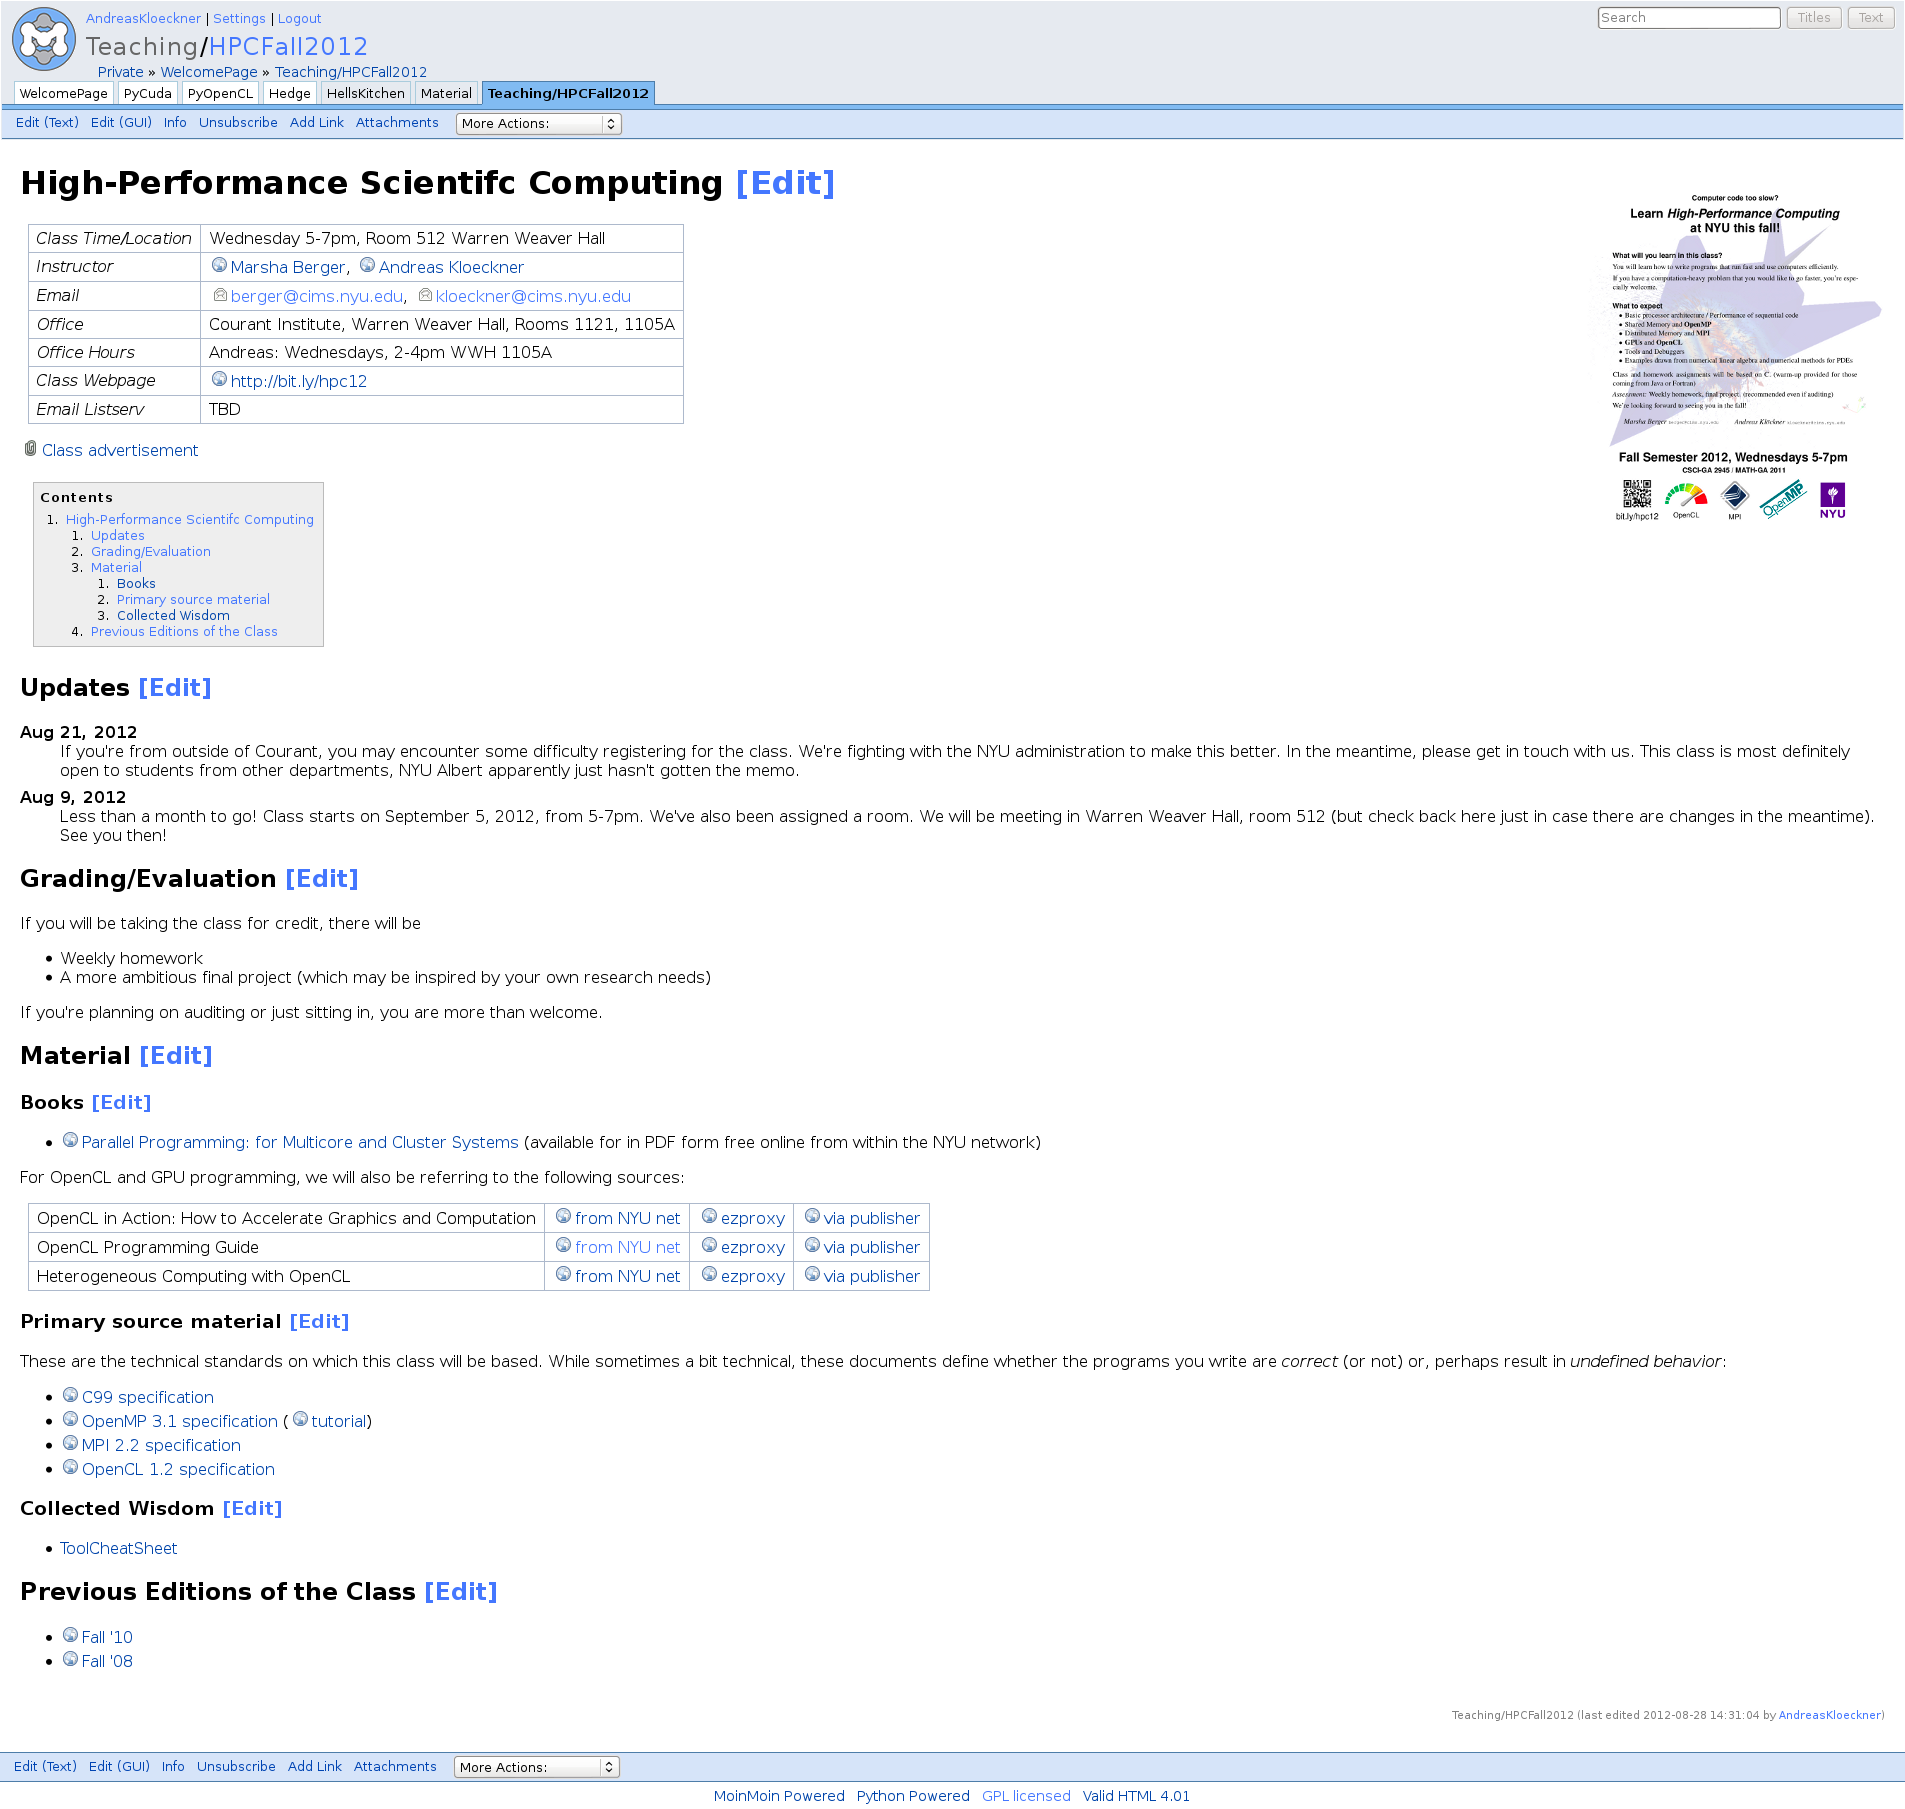
\includegraphics[width=\textwidth]{hpc-web-screenshot.png}
    \column{0.4\textwidth}
      \Huge
      \href{http://bit.ly/hpc12}{bit.ly/hpc12}
  \end{columns}
\end{frame}
% -----------------------------------------------------------------------------
\begin{frame}{Book 1}
  \begin{center}
    
\includegraphics[height=7cm]{rauber-ruenger.jpeg}
  \end{center}
\end{frame}
% -----------------------------------------------------------------------------
\begin{frame}{Books 2--4}
  \begin{center}
    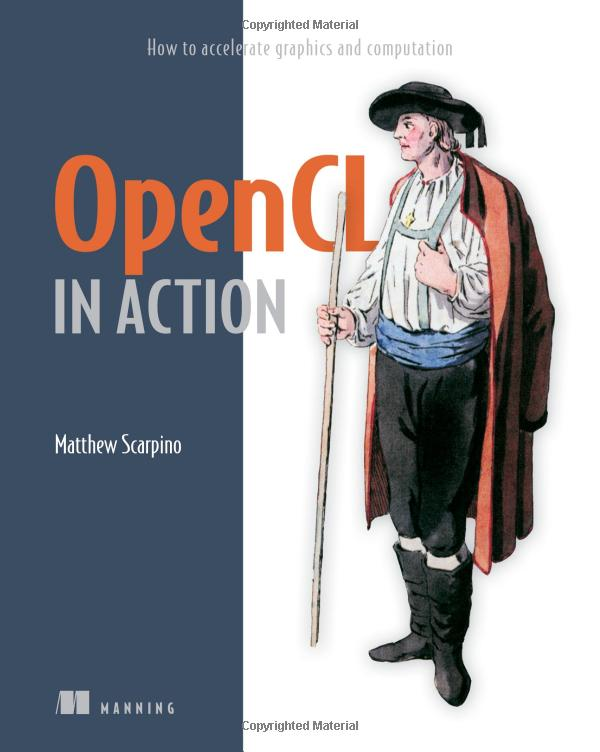
\includegraphics[height=7cm]{scarpino-opencl.jpeg}
  \end{center}
\end{frame}
% -----------------------------------------------------------------------------
\begin{frame}{Books 2--4}
  \begin{center}
    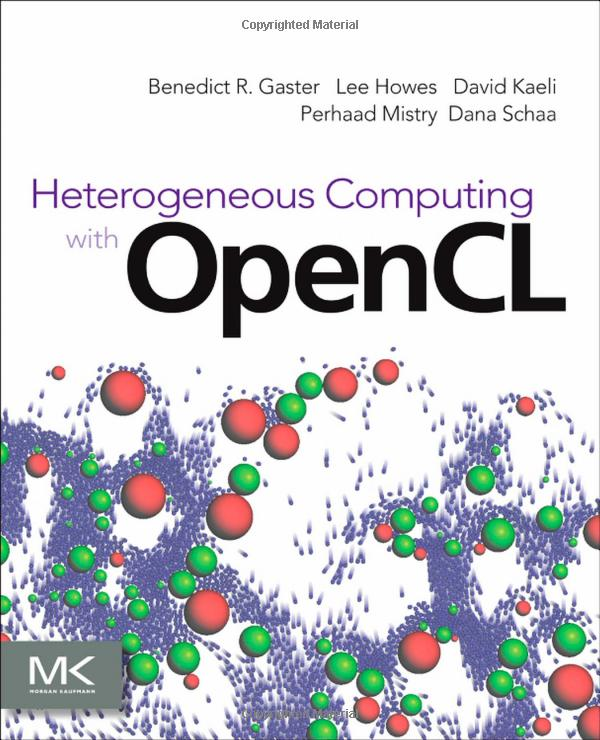
\includegraphics[height=7cm]{gaster-opencl.jpeg}
  \end{center}
\end{frame}
% -----------------------------------------------------------------------------
\begin{frame}{Grading}
  \Large
  \begin{itemize}
    \item 60\% Weekly homework
    \item 40\% Final project
  \end{itemize}
\end{frame}
% -----------------------------------------------------------------------------
\begin{frame}{Books 2--4}
  \begin{center}
    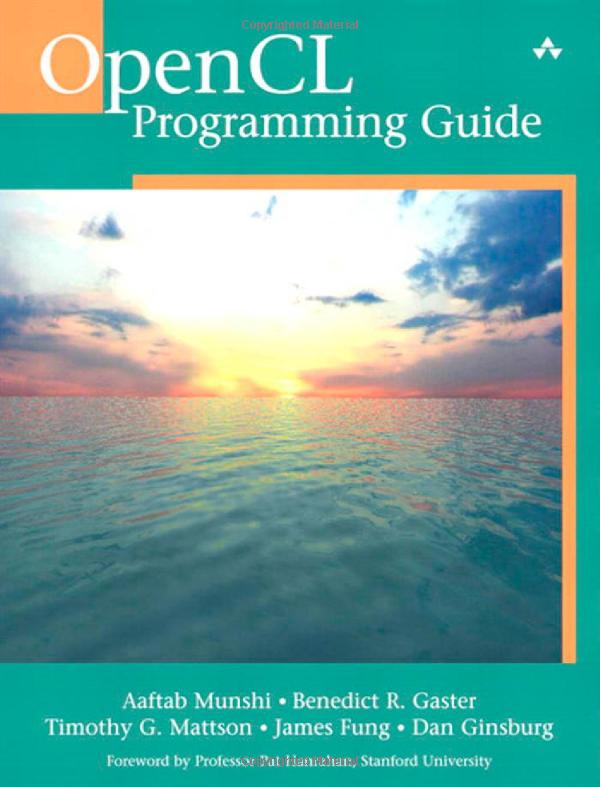
\includegraphics[height=7cm]{munshi-opencl.jpeg}
  \end{center}
\end{frame}
% -----------------------------------------------------------------------------
\begin{frame}{Listserv}
  \begin{center}
    \Huge
    \href{mailto:hpc12@tiker.net}{hpc12@tiker.net}
  \end{center}
\end{frame}
% -----------------------------------------------------------------------------
\begin{frame}{Smile! You're on camera}
  \begin{center}
    \includegraphics[height=5cm]{camera.jpeg}

    Lecture video will be posted soon after each class.
  \end{center}
\end{frame}
\addimgcredit{Camera: sxc.hu/Kolobsek}
% }}}
% -----------------------------------------------------------------------------
\section{HPC: A look around}
% -----------------------------------------------------------------------------
% {{{
\begin{frame}{Key Realization}
  \begin{center}
    \Huge
    My computer is too slow.
  \end{center}
  \uncover<2>{
    \begin{tikzpicture} [overlay]
      \node [above left=10mm of current page.south east,
      draw,drop shadow,fill=white,inner sep=5mm,thick]
        {
          Maybe it'll get faster if I wait long enough?
        } ;
    \end{tikzpicture}
  }
\end{frame}
% -----------------------------------------------------------------------------
\begin{frame}{Moore's law}
  \begin{center}
    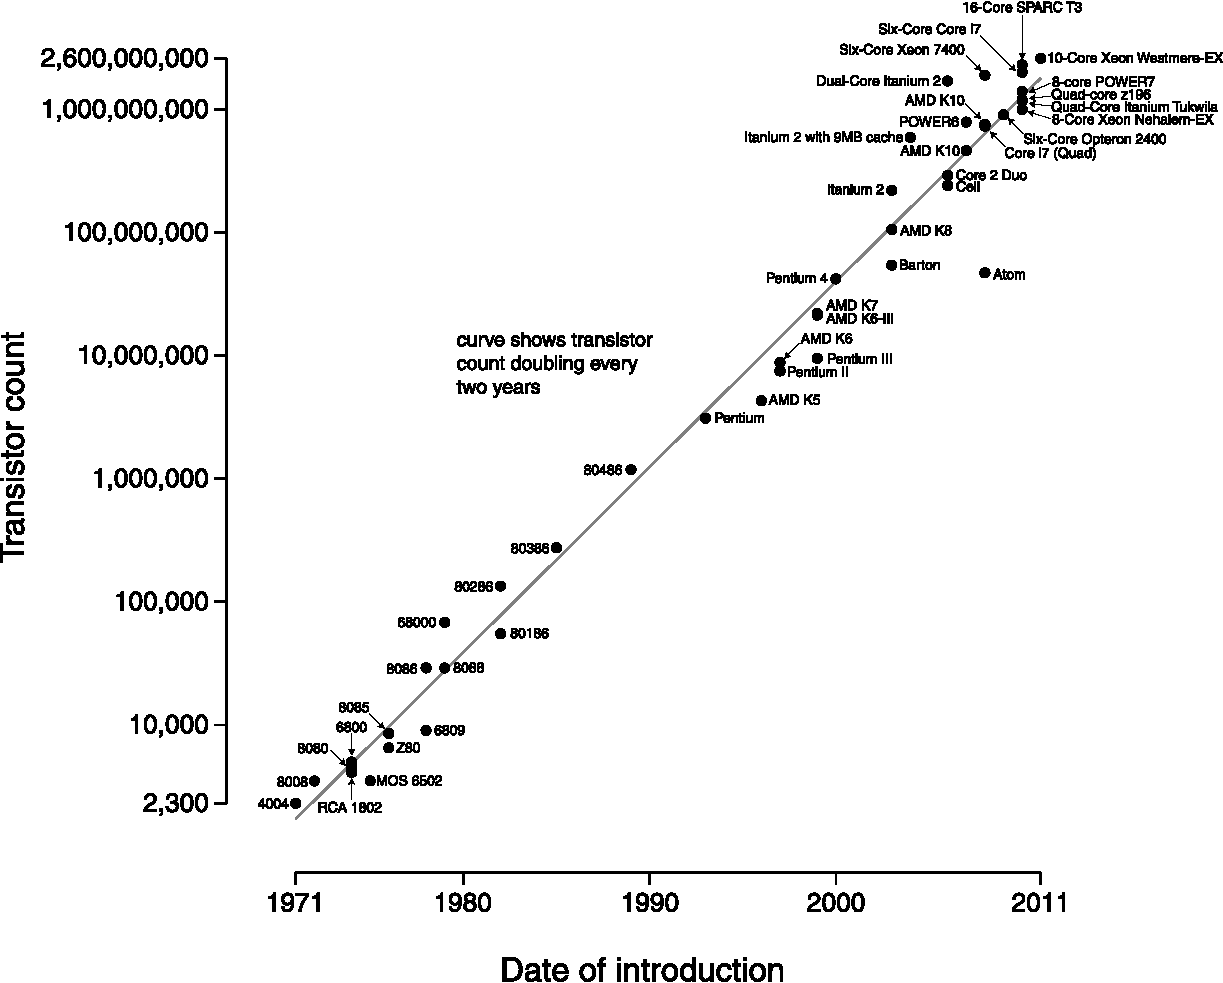
\includegraphics[height=8cm]{moores-law.pdf}
  \end{center}
  \uncover<2>{
    \begin{tikzpicture} [overlay]
      \node [above left=10mm of current page.south east,
      draw,drop shadow,fill=white,inner sep=5mm,thick]
        {
          \textbf{Issue:} More transistors $\ne$ faster
        } ;
    \end{tikzpicture}
  }
\end{frame}
\addimgcredit{Moore's law: Wikipedia}
% -----------------------------------------------------------------------------
% moore's law
% but: dennard scaling
% but: people don't think in parallel
% MANY types of parallelism (in hw)
% MANY ways to express parallelism
% annoying
% but: the only way to get more perf!
% venn: correct, fast
% need to know correct before fast
%   -> that's how we'll do business

% shared vs distributed memory
% hpc as a spectator sport

% amdahl, speedup, efficiency
% Flynn: +SPMD +SIMT
% }}}
% -----------------------------------------------------------------------------
\section{A taste of what's to come}
% -----------------------------------------------------------------------------
% {{{
% vector addition through the paradigms
% }}}

\questionframe{}
\imagecreditslide

\end{document}
% vim: foldmethod=marker
